\documentclass[mathserif]{beamer}
\usepackage[utf8]{inputenc}
\usepackage{amsmath}
\usepackage{amsfonts}
\usepackage{amssymb}
\usepackage{arydshln}
\usepackage{graphicx}
\usepackage{float}
\usepackage{picture}
\usepackage{dcolumn}
 
%Information to be included in the title page:
\title{Linux for Embedded Objects 2}
\author{Thomas S. Christensen, Mikkel S. Jaedicke}
\institute{University of Southern Denmark}
\date{Jun, 2017} 
 
\usetheme{Berkeley}
\usecolortheme{seagull} 

\begin{document}
 
\begin{frame}
	\section{Disposition}
	\frametitle{Linux on the Zynq Platform}
	Disposition:
	\begin{itemize}
		\item \textbf{Motivation}
		\item \textbf{Zynq Platform}
		\item \textbf{Boot Process}
		\item \textbf{Cross Compilation}
	\end{itemize}
\end{frame}

\begin{frame}
	\section{Motivation}
	\frametitle{Motivation}
	\centering
	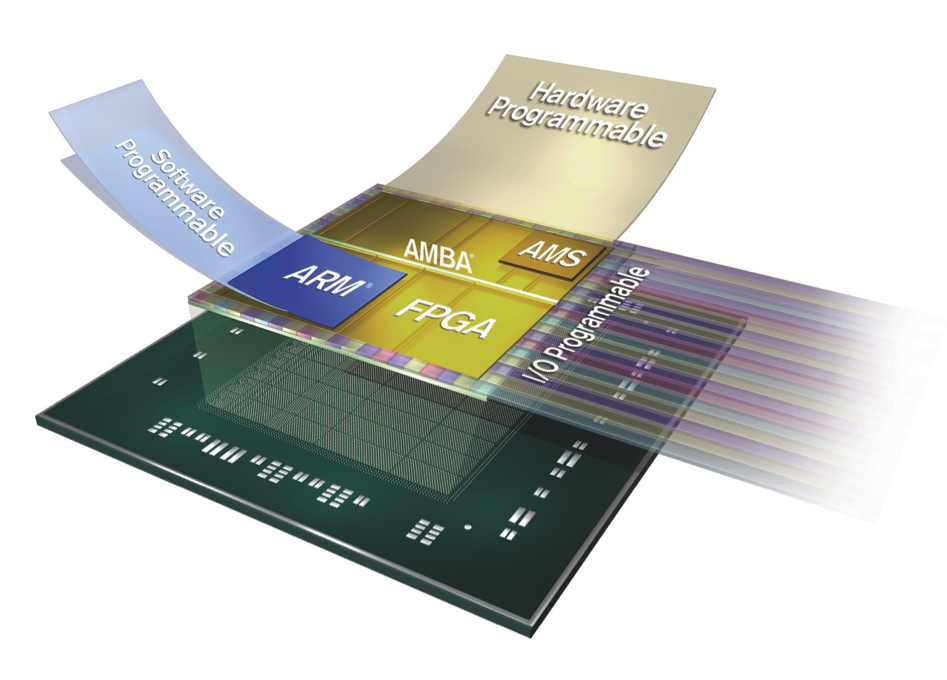
\includegraphics[width=.35\linewidth]{graphics/zynq.png}
	\begin{itemize}
		\item Customizability
		\item Efficiency on a changing platform
		\item Knowledge about the platform
	\end{itemize}
\end{frame}

\begin{frame}
	\section{Zynq Platform}
	\frametitle{Zynq Platform}
	\centering
	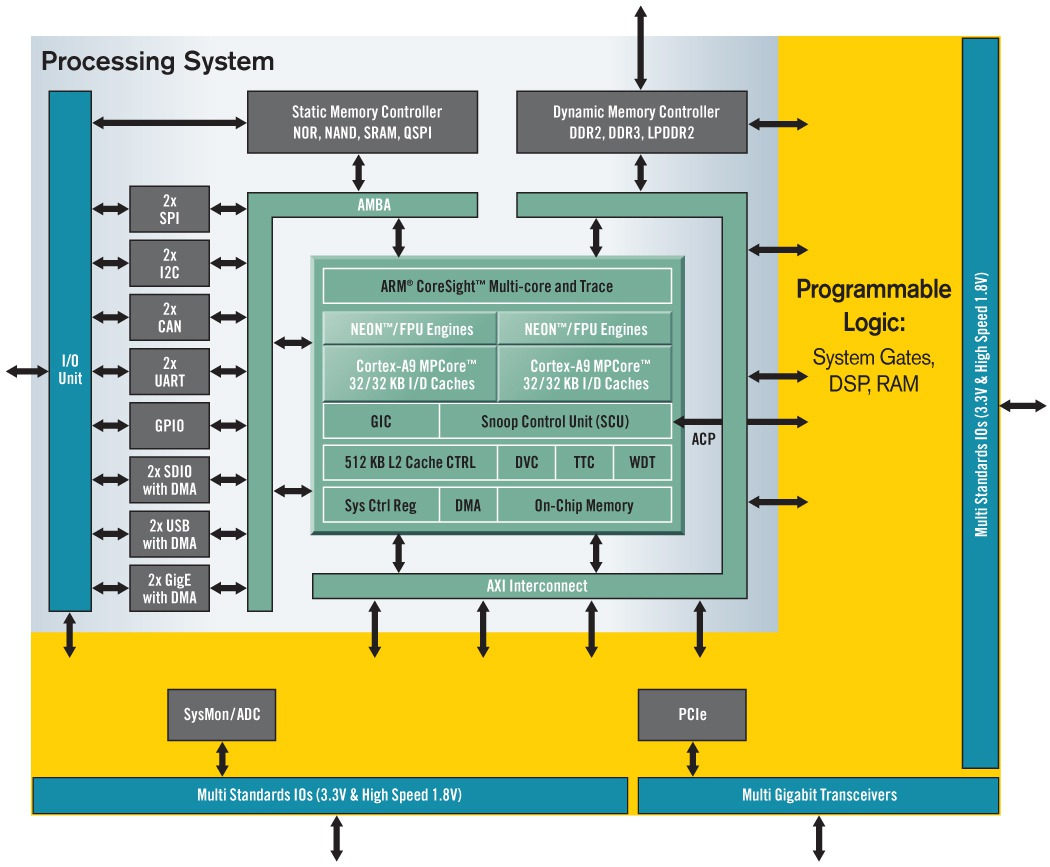
\includegraphics[width=.75\linewidth]{graphics/zynq_architecture}
\end{frame}

\begin{frame}
	\section{Boot Process}
	\frametitle{The Zynq Boot Process}
	\centering
	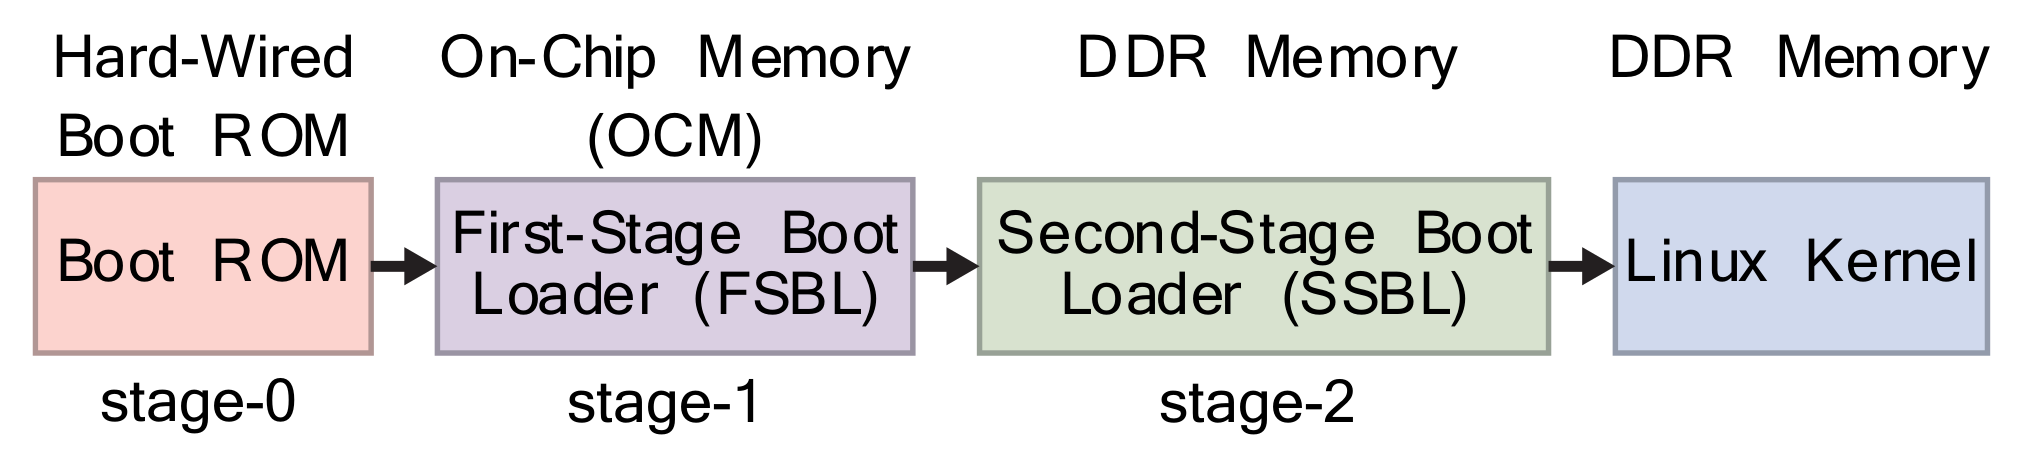
\includegraphics[width=\linewidth]{graphics/zynq_boot_process}
\end{frame}

\begin{frame}
	\frametitle{Stage 0 - Boot ROM}
	\centering
	\begin{itemize}
		\item Hardcoded
		\item Determines the boot mode
		\item Loads FSBL into OCM
	\end{itemize}
\end{frame}

\begin{frame}
	\frametitle{Stage 1 - First-Stage Boot Loader}
	\centering
	\begin{itemize}
		\item PS and PL configuration
		\item Loads SSBL into DDR RAM
	\end{itemize}
\end{frame}

\begin{frame}
	\frametitle{Stage 2 - Second-Stage Boot Loader}
	\centering
	\begin{itemize}
		\item Bare-metal application
		\item U-Boot
		\item Loads device tree to memory
		\item Loads the kernel image into memory
		\item Initialises execution of the Linux kernel
	\end{itemize}
\end{frame}

\begin{frame}
	\frametitle{The Boot Image}
	\centering
	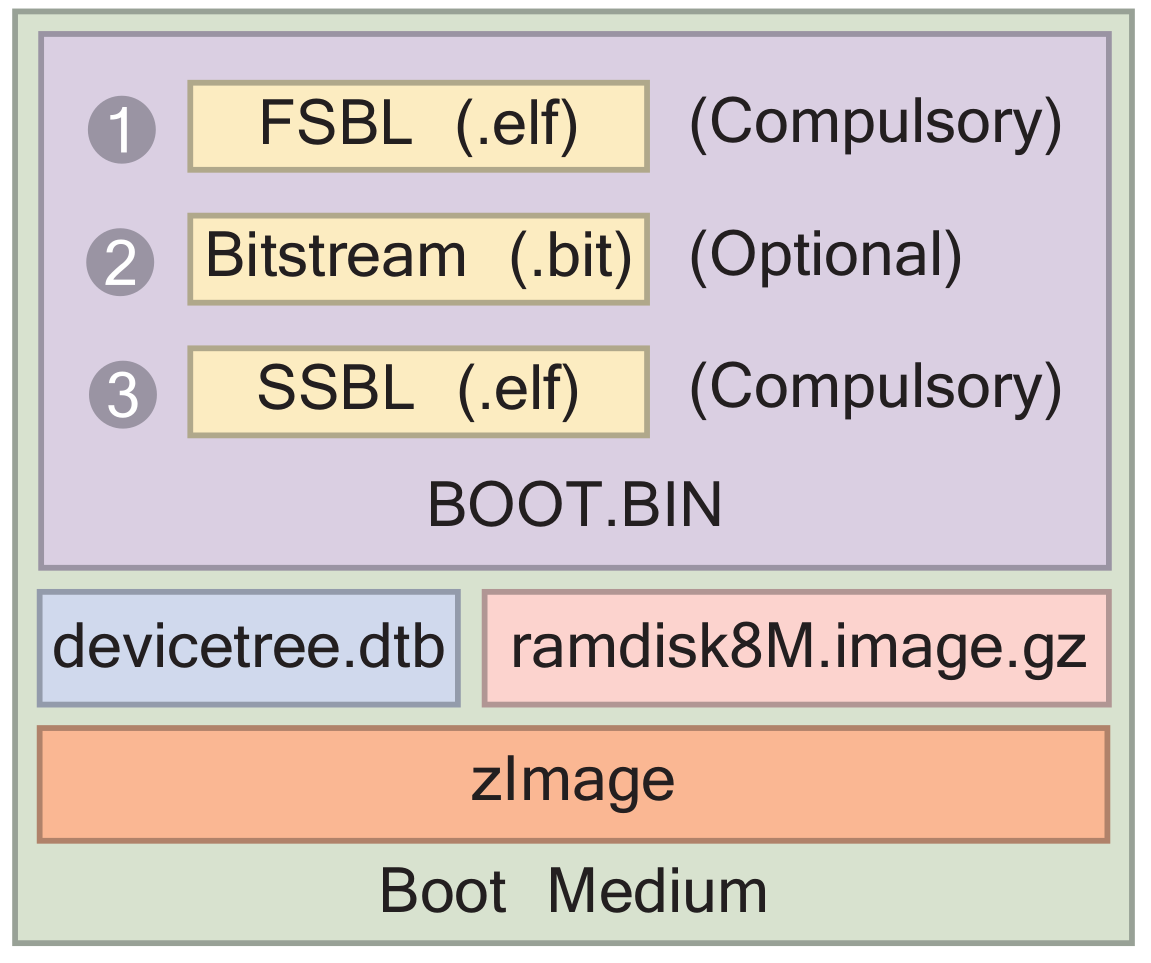
\includegraphics[width=.65\linewidth]{graphics/boot_image}
\end{frame}

\begin{frame}
	\section{Cross Compilation}
	\frametitle{Cross Compilation}
	\centering
	\begin{itemize}
		\item Why?
		\item The cross compilation toolchain
		\item Compilation of userspace software
		\item Make!
	\end{itemize}
\end{frame}

\begin{frame}
	\frametitle{Cross Compilation of Kernel Modules}
	\centering
	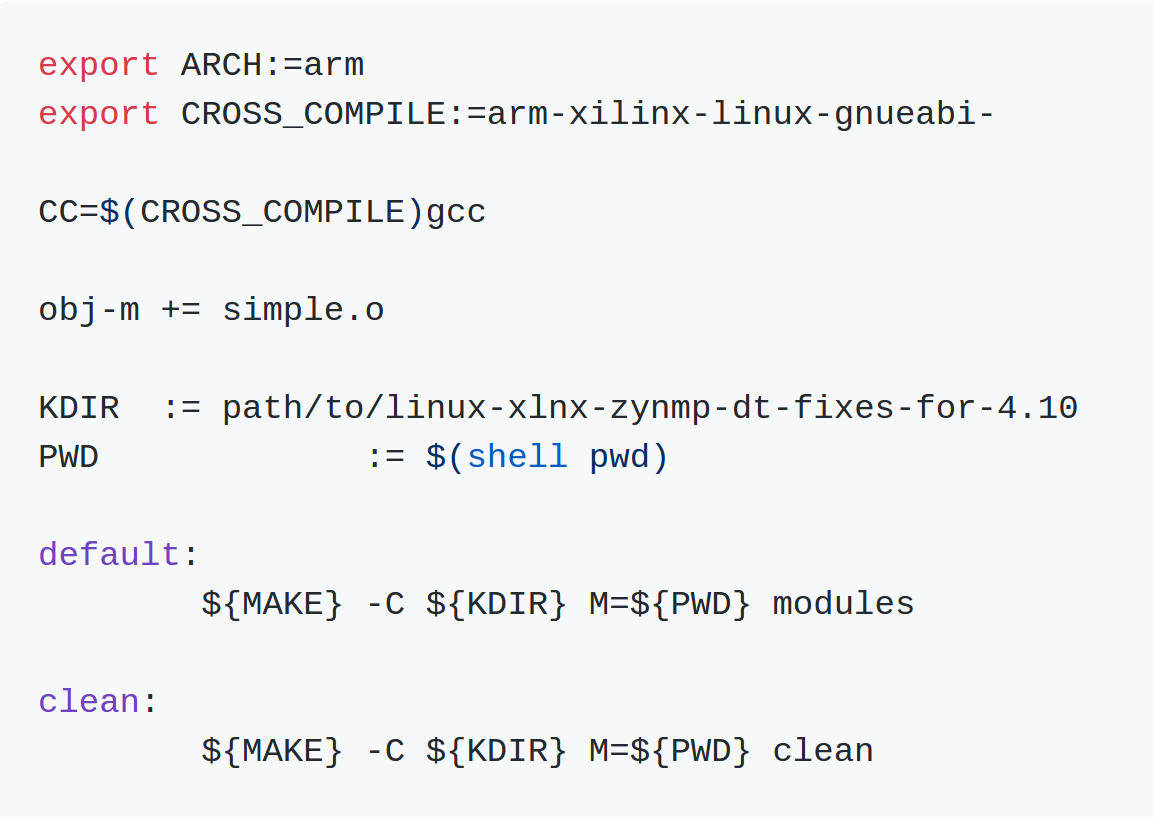
\includegraphics[width=.85\linewidth]{graphics/makefile}
\end{frame}
\end{document}